\documentclass{article}

\usepackage{geometry}
 \geometry{
 a4paper,
 total={170mm,257mm},
 left=20mm,
 top=20mm
 }
\usepackage{float}
\usepackage{graphicx}
\usepackage{indentfirst}
\usepackage{hyperref}

\graphicspath{ {./images/} }
\renewcommand*\contentsname{Daftar Isi}
\renewcommand{\figurename}{Figur}
\renewcommand{\tablename}{Tabel}

\begin{document}
	\begin{titlepage}
		\begin{center}
			
			\null
			{
				\huge \bfseries Tugas Praktikum Pengembangan Perangkat Lunak}\\
			[1cm]
			{\LARGE Statechart Diagram KataHati}\\
			
			\vspace{2cm}
			
			\begin{figure}[H]
				\centering
				
\includegraphics[width=200px]{/HitamPutih.jpg}
			\end{figure}
			
			\vspace{3cm}
			
			{\Large 
				Disusun oleh Kelompok YapaYapaHuy} {\Large :\\
				\vspace{0.5cm}
				Ardacandra Subiantoro (18/427572/PA/18532)\\
				Chrystian (18/430257/PA/18770)\\
				Juandito Batara Kuncoro (18/427582/PA/18542)\\
			}
			
			
			\vspace{2cm}
			
			{\normalsize \bfseries
				PROGRAM STUDI S1 ILMU KOMPUTER\\
				DEPARTEMEN ILMU KOMPUTER DAN ELEKTRONIKA\\
				FAKULTAS MATEMATIKA DAN ILMU PENGETAHUAN ALAM\\
				UNIVERSITAS GADJAH MADA\\
				YOGYAKARTA\\
				\vspace{0.2cm}
				2020
			}
			
		\end{center}
	\end{titlepage}

	\newpage
	\pagenumbering{arabic}
	
	\section{Statechart Diagram}
	\begin{figure}[H]
		\centering
		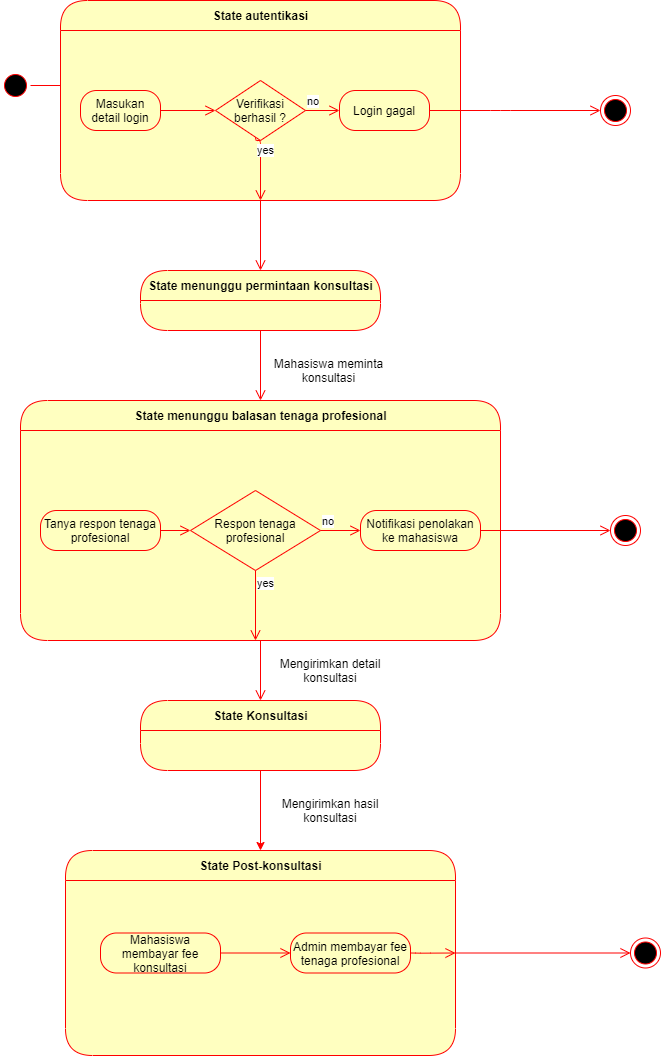
\includegraphics[height=650px]{/state_diagram.png}
	\end{figure}
\end{document}